\documentclass[14pt, a4paper]{extarticle}
\usepackage{GOST}
\usepackage{array}
\usepackage{verbatim}
\usepackage[detect-all]{siunitx}
\usepackage{amsmath}
\usepackage{amssymb}
\usepackage[utf8]{inputenc}
\usepackage{hyperref}
\usepackage{tempora}

\makeatletter
\renewcommand\@biblabel[1]{#1.}
\makeatother

\usepackage{listings}
\lstset{ 
	language=C,
	basicstyle=\small, 
	numbers=left, 
	numberstyle=\tiny,
	stepnumber=1,
	numbersep=5pt,
	showspaces=false,            
	showstringspaces=false,      
	showtabs=false,             
	frame=single,            % рисовать рамку вокруг кода
	tabsize=4,      
	commentstyle=\color{green},
	keywordstyle=\color{blue}\textbf,
	numberstyle=\scriptsize\color{gray}, % the style that is used for the line-numbers
	rulecolor=\color{black},
	captionpos=t,
	breaklines=true,         % автоматически переносить строки 
	breakatwhitespace=false, % переносить строки по пробелу
	%escapeinside={\#*}{*)} 
}


\usepackage{pgfplots}
\usepackage{filecontents}
\usetikzlibrary{datavisualization}
\usetikzlibrary{datavisualization.formats.functions}

\begin{document}
	
\begin{table}[ht]
	\centering
	\begin{tabular}{|c|p{400pt}|} 
		\hline
		\begin{tabular}[c]{@{}c@{}} 
\includegraphics[scale=1]{source/b_logo.jpg} \\\end{tabular} &
		\footnotesize\begin{tabular}[c]{@{}c@{}}\textbf{Министерство~науки~и~высшего~образования~Российской~Федерации}\\\textbf{Федеральное~государственное~бюджетное~образовательное~учреждение}\\\textbf{~высшего~образования}\\\textbf{«Московский~государственный~технический~университет}\\\textbf{имени~Н.Э.~Баумана}\\\textbf{(национальный~исследовательский~университет)»}\\\textbf{(МГТУ~им.~Н.Э.~Баумана)}\\\end{tabular}  \\
		\hline
	\end{tabular}
\end{table}
\noindent\rule{\textwidth}{4pt}
\noindent\rule[14pt]{\textwidth}{1pt}
\hfill 
\noindent
\makebox{ФАКУЛЬТЕТ~}%
\makebox[\textwidth][l]{\underline{~«Информатика и системы управления»~~~~~~~~~~~~~~~~~~~~~~~~~~~~~~~~~}}%
\\
\noindent
\makebox{КАФЕДРА~}%
\makebox[\textwidth][l]{\underline{~«Программное обеспечение ЭВМ и информационные технологии»~}}%
\\

\begin{center}
	\vspace{1.5cm}
	{\bf\huge Отчёт\par}
	{\bf\Large по лабораторной работе № 5\par}
	\vspace{0.7cm}
\end{center}


\noindent
\makebox{\large{\bf Название:}~~~}
\makebox[\textwidth][l]{\large\underline{~Взаимодействие параллельных процессов~}}\\

\noindent
\makebox{\large{\bf Дисциплина:}~~~}
\makebox[\textwidth][l]{\large\underline{~Операционные системы~~~~~~~~~~~~~~~~~~~~~~~~~~}}\\

\vspace{1.5cm}
\noindent
\begin{tabular}{l c c c c c}
	Студент      & ~ИУ7-55Б~               & \hspace{2.5cm} & \hspace{2cm}                 & &  Д.О. Склифасовский \\\cline{2-2}\cline{4-4} \cline{6-6} 
	\hspace{3cm} & {\footnotesize(Группа)} &                & {\footnotesize(Подпись, дата)} & & {\footnotesize(И.О. Фамилия)}
\end{tabular}

\noindent
\begin{tabular}{l c c c c}
	Преподаватель & \hspace{5cm}   & \hspace{2cm}                 & & ~~~~~~Н.Ю. Рязанова~~~~~~\\\cline{3-3} \cline{5-5} 
	\hspace{3cm}  &                & {\footnotesize(Подпись, дата)} & & {\footnotesize(И.О. Фамилия)}
\end{tabular}

\vspace{0.6cm}
\begin{center}	
	\vfill
	\large \textit {Москва, 2020}
\end{center}

\thispagestyle {empty}
\pagebreak

\clearpage
\tableofcontents

\clearpage
\section{Задание}
Написать программу, реализующую задачу «Производство-потребление» по алгоритму Э. Дейкстры с тремя семафорами: двумя считающими и одним бинарным. В программе должно создаваться не менее 3х процессов - производителей и 3х процессов – потребителей. В программе надо обеспечить случайные задержки выполнения созданных процессов. В программе для взаимодействия производителей и потребителей буфер создается в разделяемом сегменте. Обратите внимание на то, чтобы не работать с одиночной переменной, а работать именно с буфером, состоящим их N ячеек по алгоритму. Производители в ячейки буфера записывают буквы алфавита по порядку. Потребители считывают символы из доступной ячейки. После считывания буквы из ячейки следующий потребитель может взять букву из следующей ячейки. \par

\textbf{Программа:}
\begin{lstlisting}[label=task1, caption=Задание 1]
#include <stdio.h>
#include <stdlib.h>
#include <unistd.h>
#include <sys/types.h>
#include <sys/ipc.h>
#include <sys/sem.h>
#include <sys/shm.h>
#include <sys/wait.h>
#include <sys/stat.h>
#include <time.h>

#define SIZE 24

#define FULL 0
#define EMPTY 1
#define BIN 2

#define PROD 3
#define CONS 3

char* shared_buffer = NULL;
char* cons_pos = 0;
char* prod_pos = 0;

char alph[] = "ABCDEFGHIJKLMNOPQRSTUVWXYZ";
int len = 26;

struct sembuf prod_start[2] = {
    {EMPTY, -1, 0},
    {BIN, -1, 0}
};
struct sembuf prod_stop[2] = {
    {BIN, 1, 0},
    {FULL, 1, 0}
};

struct sembuf cons_start[2] = {
    {FULL, -1, 0},
    {BIN, -1, 0}
};
struct sembuf cons_stop[2] = {
    {BIN, 1, 0},
    {EMPTY, 1, 0}
};

int perms = S_IRWXU | S_IRWXG | S_IRWXO;

int get_sem() 
{
    int sem = semget(IPC_PRIVATE, 3, IPC_CREAT | perms);
    if (sem == -1)
    {
        perror("sem\n");
        exit(1);
    }
    int s1 = semctl(sem, FULL, SETVAL, 0);
    int s2 = semctl(sem, EMPTY, SETVAL, SIZE);
    int s3 = semctl(sem, BIN, SETVAL, 1);
    
    return sem;
}

int get_shared_memory()
{
    int shared_memory = shmget(IPC_PRIVATE, (SIZE + 2) * sizeof(char), IPC_CREAT | perms);
    if (shared_memory == -1) 
    {
        perror("shmget\n");
        exit(1);
    }

    prod_pos = (char*)shmat(shared_memory, 0, 0);
    if (prod_pos == (char*)-1) 
    {
        perror("shmat\n");
        exit(1);
    }
    cons_pos = prod_pos + sizeof(char);
    shared_buffer = cons_pos + sizeof(char);
    
    return shared_memory;
}

void producer(int sem, int id)
    {
    while(1) 
    {    
        if (semop(sem, prod_start, 2) == -1)
        {
            perror("semop\n");
            exit(1);
        }

        shared_buffer[*prod_pos] = alph[*prod_pos];
        printf("Producer %d: %c\n", id, alph[*prod_pos]);

        if (++(*prod_pos) == len) 
            (*prod_pos) = 0;

        if (semop(sem, prod_stop, 2) == -1)
        {
            perror("semop\n");
            exit(1);
        }

        sleep(rand() % 5);
    }
}

void consumer(int sem, int id)
{
    while(1) 
    {
        if (semop(sem, cons_start, 2) == -1)
        {
            perror("semop\n");
            exit(1);
        }

        printf("Consumer %d: %c\n", id, shared_buffer[*cons_pos]);
        
        if (++(*cons_pos) == len)
            (*cons_pos) = 0;

        if (semop(sem, cons_stop, 2) == -1)
        {
            perror("semop\n");
            exit(1);
        }

        sleep(rand() % 5);
    }
}

void fork_proc(void (*func)(int sem, int id), int sem, int count)
{
    for (int i = 0; i < count; i++) 
    {
        pid_t pid = fork();

        if (pid == -1)
        {
            perror("fork");
            exit(1);
        }

        if (pid == 0) 
        {
            func(sem, i + 1);
            exit(0);
        }
    }
}

void catch_signal(int signalNum)
{
    printf("Catched\n");
}

int main()
{
    int shared_memory = get_shared_memory();
    int sem = get_sem();

    fork_proc(producer, sem, PROD);
    fork_proc(consumer, sem, CONS);

    signal(SIGINT, catch_signal);

    for (int i = 0; i < PROD + CONS; i++)
    {
        int status;
        wait(&status);
    }

    shmctl(shared_memory, IPC_RMID, NULL);
    semctl(sem, BIN, IPC_RMID, 0);

    return 0;
}

\end{lstlisting}
\textbf{Результат работы программы:}\par
\begin{figure}[h!]
	\centering
	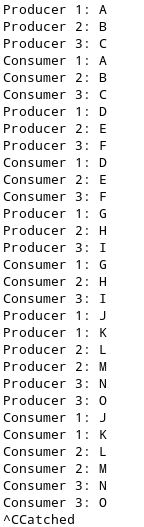
\includegraphics[scale=1]{source/1.png}
	\caption{Результат работы программы}
	\label{Example1}
\end{figure}\par

\newpage
\section{Задание}
Написать программу, реализующую задачу «Читатели – писатели» по монитору Хоара с четырьмя функциями: Начать\_чтение, Закончить\_чтение, Начать\_запись, Закончить\_запись. В программе всеми процессами разделяется одно единственное значение в разделяемой памяти. Писатели ее только инкрементируют, читатели могут только читать значение.\par
Для реализации взаимоисключения используются семафоры\par
\textbf{Программа:}
\begin{lstlisting}[label=task1, caption=Задание 2]
#include <stdio.h>
#include <stdlib.h>
#include <unistd.h>
#include <sys/types.h>
#include <sys/ipc.h>
#include <sys/sem.h>
#include <sys/shm.h>
#include <sys/wait.h>
#include <sys/stat.h>
#include <time.h>
#define ACTIVE_WRITER 0
#define WAITING_WRITER 1
#define ACTIVE_READER 2
#define WAITING_READER 3

int* shared_buffer = NULL;

struct sembuf startread[5] =
{
    {ACTIVE_WRITER, 0, 0},
    {WAITING_WRITER, 0, 0},
    {WAITING_READER, 1, 0},
    {ACTIVE_READER, 1, 0},
    {WAITING_READER, -1, 0}
};
struct sembuf stopread[1] = 
{
    {ACTIVE_READER, -1, 0}
};

struct sembuf startwrite[5] =
{
    {ACTIVE_READER, 0, 0},
    {ACTIVE_WRITER, 0, 0},
    {WAITING_WRITER, 1, 0},
    {ACTIVE_WRITER, 1, 0},
    {WAITING_WRITER, -1, 0}
};
struct sembuf stopwrite[1] = 
{
    {ACTIVE_WRITER, -1, 0}
};

int perms = S_IRWXU | S_IRWXG | S_IRWXO;

int readers = 5;
int writers = 3;

int get_sem() 
{
    int sem = semget(IPC_PRIVATE, 5, IPC_CREAT | perms);
    if (sem == -1)
    {
        perror("sem\n");
        exit(1);
    }
    int s1 = semctl(sem, ACTIVE_WRITER, SETVAL, 0);
    int s2 = semctl(sem, ACTIVE_READER, SETVAL, 0);
    int s3 = semctl(sem, WAITING_WRITER, SETVAL, 0);
    int s4 = semctl(sem, WAITING_READER, SETVAL, 0);

    return sem;
}

int get_shared_memory()
{
    int shared_memory = shmget(IPC_PRIVATE, sizeof(int), IPC_CREAT | perms);
    if (shared_memory == -1) 
    {
        perror("shmget\n");
        exit(1);
    }

    shared_buffer = (int*)shmat(shared_memory, 0, 0);
    if (shared_buffer == (int*)-1) 
    {
        perror("shmat\n");
        exit(1);
    }
    
    *shared_buffer = 0;
    
    return shared_memory;
}

void start_read(int sem)
{
    if (semop(sem, startread, 5) == -1)
    {
        perror("semop\n");
        exit(1);
    }
}

void stop_read(int sem)
{
    if (semop(sem, stopread, 1) == -1)
    {
        perror("semop\n");
        exit(1);
    }
}

void start_write(int sem)
{
    if (semop(sem, startwrite, 5) == -1)
    {
        perror("semop\n");
        exit(1);
    }
}

void stop_write(int sem)
{
    if (semop(sem, stopwrite, 1) == -1)
    {
        perror("semop\n");
        exit(1);
    }
}

void writer(int sem, int id) 
{
    while (1)
    {
        start_write(sem);

        *shared_buffer += 1;
        printf("Writer %d: %d\n", id, *shared_buffer);

        stop_write(sem);

        sleep(rand() % 5);
    }
}

void reader(int sem, int id) 
{
    while (1)
    {
        start_read(sem);

        printf("Reader %d: %d\n", id, *shared_buffer);

        stop_read(sem);

        sleep(rand() % 5);
    }
}

void fork_proc(void (*func)(int sem, int id), int sem, int count)
{
    for (int i = 0; i < count; i++) 
    {
        pid_t pid = fork();

        if (pid == -1)
        {
            perror("fork");
            exit(1);
        }

        if (pid == 0) 
        {
            func(sem, i + 1);
            exit(0);
        }
    }
}

void catch_signal(int signalNum)
{
    printf("Catched\n");
}

int main()
{
    srand(time(NULL));
    int shared_memory = get_shared_memory();
    int sem = get_sem();

    fork_proc(writer, sem, writers);
    fork_proc(reader, sem, readers);
    
    signal(SIGINT, catch_signal);

    for (int i = 0; i < writers + readers; i++)
    {
        int status;
        wait(&status);
    }

    shmctl(shared_memory, IPC_RMID, NULL);

    return 0;
}

\end{lstlisting}
\textbf{Результат работы программы:}\par
\begin{figure}[h!]
	\centering
	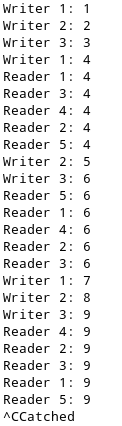
\includegraphics[scale=1]{source/2.png}
	\caption{Результат работы программы}
	\label{Example2}
\end{figure}\par
\end{document}